\documentclass[12pt, oneside]{article}

\usepackage[letterpaper, scale=0.89, centering]{geometry}
\usepackage{fancyhdr}
\setlength{\parindent}{0em}
\setlength{\parskip}{1em}

\usepackage{tikz}
\usetikzlibrary{automata,positioning,arrows}

\pagestyle{fancy}
\fancyhf{}
\renewcommand{\headrulewidth}{0pt}
\rfoot{\href{https://creativecommons.org/licenses/by-nc-sa/2.0/}{CC BY-NC-SA 2.0} Version \today~(\thepage)}

\usepackage{amssymb,amsmath,pifont,amsfonts,comment,enumerate,enumitem}
\usepackage{currfile,xstring,hyperref,tabularx,graphicx,wasysym}
\usepackage[labelformat=empty]{caption}
\usepackage{xcolor}
\usepackage{multicol,multirow,array,listings,tabularx,lastpage,textcomp,booktabs}

\lstnewenvironment{algorithm}[1][] {   
    \lstset{ mathescape=true,
        frame=tB,
        numbers=left, 
        numberstyle=\tiny,
        basicstyle=\rmfamily\scriptsize, 
        keywordstyle=\color{black}\bfseries,
        keywords={,procedure, div, for, to, input, output, return, datatype, function, in, if, else, foreach, while, begin, end, }
        numbers=left,
        xleftmargin=.04\textwidth,
        #1
    }
}
{}

\newcommand\abs[1]{\lvert~#1~\rvert}
\newcommand{\st}{\mid}

\newcommand{\cmark}{\ding{51}}
\newcommand{\xmark}{\ding{55}}
 
\begin{document}
\begin{flushright}
    \StrBefore{\currfilename}{.}
\end{flushright} 
\subsection*{Week 5 at a glance}

\subsubsection*{Textbook reading: Section 2.2, 2.1.}

\vspace{-20pt}

Before Monday, read Theorem 2.20.

Before Wednesday, read Example 2.18 (page 114).

Before Friday, read Figure 3.1.

For Week 6 Monday: Page 165-166 Introduction to Section 3.1.

\vspace{-20pt}

\subsubsection*{We will be learning and practicing to:}
\vspace{-20pt}

\begin{itemize}
    \item Clearly and unambiguously communicate computational ideas using appropriate formalism. Translate across levels of abstraction.
    \begin{itemize}
        \item Describe and use models of computation that don't involve state machines.
        \begin{itemize}
            \item {\bf Use context-free grammars and relate them to languages and pushdown automata.}
        \end{itemize}
        \item Use precise notation to formally define the state diagram of a Turing machine
        \item Use clear English to describe computations of Turing machines informally.
        \begin{itemize}
            \item {\bf Design a PDA that recognizes a given language.}
         \end{itemize}
       \item Give examples of sets that are context-free (and prove that they are).
       \begin{itemize}
          \item {\bf State the definition of the class of context-free languages}
          \item {\bf Explain the limits of the class of context-free languages}
          \item {\bf Identify some context-free sets and some non-context-free sets}
       \end{itemize}
    \end{itemize}
    \item Know, select and apply appropriate computing knowledge and problem-solving techniques. 
    Reason about computation and systems.
    \begin{itemize}
        \item Describe and prove closure properties of classes of languages under certain operations.
        \begin{itemize}
            \item {\bf Apply a general construction to create a new PDA or CFG from an example one.}
            \item {\bf Formalize a general construction from an informal description of it.}
            \item {\bf Use general constructions to prove closure properties of the class of context-free langugages.}
            \item {\bf Use counterexamples to prove non-closure properties of the class of context-free langugages.}
        \end{itemize}
    \end{itemize}
\end{itemize}

\vspace{-20pt}

\subsubsection*{TODO:}
\begin{list}{\itemsep-10pt}
   \item Schedule your Test 1 Attempt 1, Test 2 Attempt 1, Test 1 Attempt 2, and Test 2 Attempt 2 times 
   at PrairieTest (http://us.prairietest.com)
   \item Review Quiz 5 on PrairieLearn (http://us.prairielearn.com), complete by Sunday 11/4/2024
\end{list}

\newpage

\section*{Monday: Context-free languages}



Warmup:   Design a CFG to generate the  language $\{a^i b^j \mid j \geq i  \geq 0\}$
  
\vfill
{\it Sample derivation:} 

\vspace{100pt}



Design a PDA to recognize the  language $\{a^i b^j \mid j \geq i  \geq 0\}$
  
\vspace{100pt}


\vfill
\newpage

{\bf Theorem  2.20}: A language is  generated by some context-free  grammar
if  and only if it is recognized by some push-down automaton.

Definition: a language is called {\bf context-free} if it is the language generated by a context-free grammar.
The class of all context-free language over a given alphabet $\Sigma$ is called {\bf CFL}.

Consequences:
\begin{itemize}
    \item Quick proof that every regular language is context free 
    \item To prove closure of the class of context-free languages under a given operation, we can choose 
    either of two modes 
    of proof (via CFGs or PDAs) depending on which is easier
    \item To fully specify a PDA we could give its $6$-tuple formal definition or we could give its input 
alphabet, stack alphabet, and state diagram.
An informal description of a PDA is a step-by-step description of how its computations 
would process input strings; the reader should be able to reconstruct the state diagram or formal 
definition precisely from such a descripton. The informal description of a PDA can refer to some 
common modules or subroutines that are computable by PDAs:
\begin{itemize}
  \item PDAs can ``test for emptiness of stack'' without providing details. 
  {\it How?} We can always push a special end-of-stack symbol, $\$$, at the start, before processing
  any input, and then use this symbol as a flag.
  \item PDAs can ``test for end of input'' without providing details.
  {\it How?} We can transform a PDA to one where accepting states are only those reachable 
  when there are no more input symbols.
\end{itemize}

\end{itemize}




\vfill

\newpage
Suppose $L_1$ and $L_2$ are context-free languages over $\Sigma$.  {\bf Goal}:  $L_1 \cup L_2$  is  also context-free.

{\it Approach 1: with  PDAs}

Let $M_1 = ( Q_1, \Sigma, \Gamma_1, \delta_1, q_1, F_1)$ and
$M_2 = ( Q_2, \Sigma, \Gamma_2, \delta_2, q_2, F_2)$ be PDAs with 
$L(M_1) =  L_1$  and  $L(M_2) = L_2$.

Define $M = $

\vfill

{\it Approach  2: with CFGs}

Let $G_1 = (V_1, \Sigma, R_1, S_1)$  and   $G_2 = (V_2, \Sigma, R_2, S_2)$  be CFGs  with
$L(G_1) =  L_1$  and  $L(G_2) = L_2$.

Define $G = $

\vfill

\newpage
Suppose $L_1$ and $L_2$ are context-free languages over $\Sigma$.  {\bf Goal}:  $L_1 \circ L_2$  is  also context-free.


{\it Approach 1: with  PDAs}

Let $M_1 = ( Q_1, \Sigma, \Gamma_1, \delta_1, q_1, F_1)$ and
$M_2 = ( Q_2, \Sigma, \Gamma_2, \delta_2, q_2, F_2)$ be PDAs with 
$L(M_1) =  L_1$  and  $L(M_2) = L_2$.

Define $M = $

\vfill

{\it Approach  2: with CFGs}

Let $G_1 = (V_1, \Sigma, R_1, S_1)$  and   $G_2 = (V_2, \Sigma, R_2, S_2)$  be CFGs  with
$L(G_1) =  L_1$  and  $L(G_2) = L_2$.

Define $G = $

\vfill

     
\newpage
\subsection*{Wednesday: Context-free and non-context-free languages}



{\it Summary}

Over a fixed alphabet $\Sigma$, a language $L$ is {\bf regular}

\vspace{-20pt}
\begin{center}
    iff it is described by some regular expression \\
    iff it is recognized by some DFA\\
    iff it is recognized by some NFA
\end{center}

Over a fixed alphabet $\Sigma$, a language $L$ is {\bf context-free}

\vspace{-20pt}
\begin{center}
    iff it is generated by some CFG\\
    iff it is recognized by some PDA
\end{center}

\vfill

{\bf Fact}: Every regular language is a context-free language.

\vfill

{\bf Fact}: There are context-free languages that are not nonregular.

\vfill

{\bf Fact}: There are countably many regular languages.

\vfill

{\bf Fact}: There are countably infinitely many context-free languages.

\vfill

{\it Consequence}: Most languages are {\bf not} context-free!

\vfill

\newpage
{\bf Examples  of non-context-free languages}

\begin{align*}
    &\{ a^n b^n c^n \mid 0 \leq n , n \in \mathbb{Z}\}\\
    &\{ a^i b^j c^k \mid 0 \leq i \leq j \leq k , i \in \mathbb{Z}, j \in \mathbb{Z}, k \in \mathbb{Z}\}\\
    &\{ ww \mid w \in \{0,1\}^* \}
\end{align*}
(Sipser Ex 2.36, Ex 2.37, 2.38)

There is a Pumping Lemma for CFL that can be used to prove a specific language is non-context-free: 
If $A$ is a context-free language, there
is a number $p$ where, if $s$ is any string in $A$ of length at least $p$, then $s$ may be divided 
into five pieces $s = uvxyz$ where (1) for each $i \geq 0$, $uv^ixy^iz \in A$, (2) $|uv|>0$, (3) $|vxy| \leq p$.
{\it We will not go into the details of the proof or application of Pumping Lemma for CFLs this quarter.}


Recall: A set $X$ is said to be {\bf closed} under an operation $OP$ if, for any elements in $X$, applying 
$OP$ to them gives an element in $X$.  


\begin{center}
\begin{tabular}{|c|l|}
\hline
True/False & Closure claim \\
\hline
True &  The set of integers is closed under multiplication. \\
& $\forall x \forall y \left( ~(x \in \mathbb{Z} \wedge y \in \mathbb{Z})\to xy \in \mathbb{Z}~\right)$ \\
\hline
True & For each set $A$, the power set of $A$ is closed under intersection. \\
& $\forall A_1 \forall A_2 \left( ~(A_1 \in \mathcal{P}(A) \wedge A_2 \in \mathcal{P}(A) \in \mathbb{Z}) \to A_1 \cap A_2 \in \mathcal{P}(A)~\right)$ \\
\hline
  & The class of regular languages over $\Sigma$ is closed under complementation. \\
  & \\
 \hline
  & The class of regular languages over $\Sigma$ is closed under union. \\
  & \\
 \hline
  & The class of regular languages over $\Sigma$ is closed under intersection. \\
  & \\
  \hline
  & The class of regular languages over $\Sigma$ is closed under concatenation. \\
  & \\
 \hline
  & The class of regular languages over $\Sigma$ is closed under Kleene star. \\
  & \\
\hline
    & The class of context-free languages over $\Sigma$ is closed under complementation. \\
  & \\
\hline
    & The class of context-free languages over $\Sigma$ is closed under union. \\
  & \\
\hline
    & The class of context-free languages over $\Sigma$ is closed under intersection. \\
  & \\
\hline
    & The class of context-free languages over $\Sigma$ is closed under concatenation. \\
  & \\
\hline
    & The class of context-free languages over $\Sigma$ is closed under Kleene star. \\
  & \\
\hline
\end{tabular}
\end{center}

 

\newpage
\subsection*{Friday: Turing machines}



We are ready to introduce a formal model that will capture a notion of general purpose computation.
\begin{itemize}
\item {\it Similar to DFA, NFA, PDA}: input will be an arbitrary string over a fixed alphabet.
\item {\it Different from NFA, PDA}: machine is deterministic.
\item {\it Different from DFA, NFA, PDA}: read-write head can move both to the left and to the right,
and can extend to the right past the original input.
\item {\it Similar to DFA, NFA, PDA}: transition function drives computation one step at a time 
by moving within a finite set of states, always starting at designated start state.
\item {\it Different from DFA, NFA, PDA}: the special states for rejecting and accepting take effect immediately.
\end{itemize}

\vspace{-10pt}

(See more details: Sipser p. 166)

\vfill

Formally: a  Turing machine is $M= (Q, \Sigma, \Gamma, \delta, q_0, q_{accept}, q_{reject})$ 
where $\delta$ is the {\bf transition function} 
\[
  \delta: Q\times \Gamma \to Q \times \Gamma \times \{L, R\}
\]
The {\bf computation} of $M$ on a string $w$ over $\Sigma$  is:

\vspace{-10pt}

\begin{itemize}
\setlength{\itemsep}{0pt}
\item Read/write head starts at leftmost position on tape. 
\item Input string is written on $|w|$-many leftmost cells of tape, 
rest of  the tape cells have  the blank symbol. {\bf Tape alphabet} 
is $\Gamma$ with $\textvisiblespace\in \Gamma$ and $\Sigma \subseteq \Gamma$.
The blank symbol $\textvisiblespace \notin \Sigma$.
\item Given current state of machine and current symbol being read at the tape head, 
the machine transitions to next state, writes a symbol to the current position  of the 
tape  head (overwriting existing symbol), and moves the tape head L or R (if possible). 
\item Computation ends {\bf if and when} machine enters either the accept or the reject state.
This is called {\bf halting}.
Note: $q_{accept} \neq q_{reject}$.
\end{itemize}

The {\bf language recognized by the  Turing machine} $M$,  is  $L(M) = \{ w \in \Sigma^* \mid w \textrm{ is accepted by } M\}$,
which is defined as
\[
  \{ w \in \Sigma^* \mid \textrm{computation of $M$ on $w$ halts after entering the accept state}\}
\]




\newpage
\begin{multicols}{2}
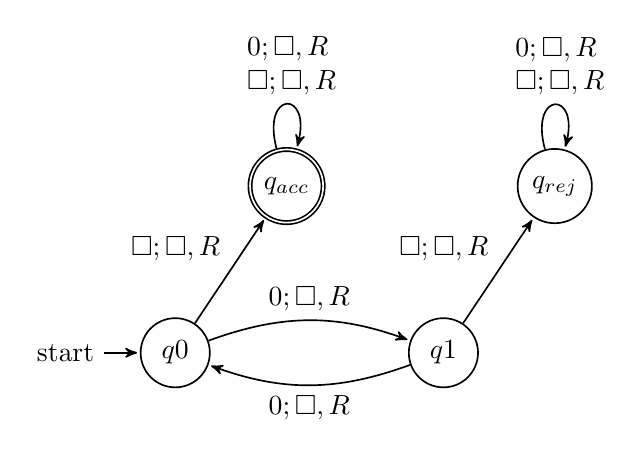
\begin{tikzpicture}[->,>=stealth',shorten >=1pt, auto, node distance=2cm, semithick]
  \tikzstyle{every state}=[text=black, fill=none]
  
  \node[initial,state] (q0)          {$q0$};
  \node[state]         (q1) [right of=q0, xshift=40pt] {$q1$};
  \node[state,accepting]         (qacc) [above right of=q0, yshift=20pt] {$q_{acc}$};
  \node[state]         (qrej) [above right of=q1,yshift=20pt] {$q_{rej}$};
  
  \path (q0) edge [bend left=0] node {$\square; \square, R$} (qacc)
      (q0) edge  [bend left=20] node {$0; \square, R$} (q1)
      (q1) edge [bend left=20] node {$0; \square, R$} (q0)
      (q1) edge [bend left=0] node {$\square; \square, R$} (qrej)
      (qacc) edge  [loop above] node {\parbox{1cm}{$0; \square, R$\newline $\square; \square, R$}} (qacc)
      (qrej) edge  [loop above] node {\parbox{1cm}{$0; \square, R$\newline $\square; \square, R$}}  (qrej)
  ;
\end{tikzpicture}
\columnbreak
Formal definition:

\vspace{10pt}

Sample computation: 

\begin{tabular}{|c|c|c|c|c|c|c|}
\hline
\multicolumn{1}{|c}{$q0\downarrow$} &  \multicolumn{6}{c|}{\phantom{A}}\\
\hline
$0$ & $0$  & $0$ & $\textvisiblespace $& $\textvisiblespace $& $\textvisiblespace $&  $\textvisiblespace $\\
\hline
\multicolumn{7}{|c|}{\phantom{A}}\\
\hline
\phantom{AA} & \phantom{AA}& \phantom{AA}& \phantom{AA}& \phantom{AA}& \phantom{AA}& \phantom{AA} \\
\hline
\multicolumn{7}{|c|}{\phantom{A}}\\
\hline
\phantom{AA} & \phantom{AA}& \phantom{AA}& \phantom{AA}& \phantom{AA}& \phantom{AA}& \phantom{AA} \\
\hline
\multicolumn{7}{|c|}{\phantom{A}}\\
\hline
\phantom{AA} & \phantom{AA}& \phantom{AA}& \phantom{AA}& \phantom{AA}& \phantom{AA}& \phantom{AA} \\
\hline
\multicolumn{7}{|c|}{\phantom{A}}\\
\hline
\phantom{AA} & \phantom{AA}& \phantom{AA}& \phantom{AA}& \phantom{AA}& \phantom{AA}& \phantom{AA} \\
\hline
\end{tabular}
\end{multicols}
\vfill

The language recognized by this machine is \ldots

\vfill
 

{\bf Describing  Turing machines} (Sipser p. 185) To define a Turing machine, we could give a 
\begin{itemize}
\item {\bf Formal definition}: the $7$-tuple of parameters including set of states, 
input alphabet, tape alphabet, transition function, start state, accept state, and reject state; or,
\item {\bf Implementation-level definition}: English prose that describes the Turing machine head 
movements relative to contents of tape, and conditions for accepting / rejecting based on those contents.
\item {\bf High-level description}: description of algorithm (precise sequence of instructions), 
without implementation details of machine. As part of this description, can ``call" and run 
another TM as a subroutine.
\end{itemize}
  
\newpage
Fix $\Sigma = \{0,1\}$, $\Gamma = \{ 0, 1, \textvisiblespace\}$ for the Turing machines with  the following state diagrams:
  
\begin{center}
  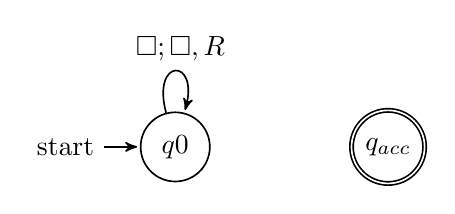
\begin{tikzpicture}[->,>=stealth',shorten >=1pt, auto, node distance=2cm, semithick]
    \tikzstyle{every state}=[text=black, fill=none]
    
    \node[initial,state] (q0)          {$q0$};
    \node[state,accepting]         (qacc) [right of=q0, xshift=20pt] {$q_{acc}$};
    
    \path (q0) edge  [loop above] node {\parbox{1cm}{$\square; \square, R$}} (q0)
    ;
  \end{tikzpicture}
\end{center}

Example of string accepted: \\
Example of string rejected: \\


Implementation-level description

\vfill

High-level description

\vfill

\begin{center}
  \begin{tikzpicture}[->,>=stealth',shorten >=1pt, auto, node distance=2cm, semithick]
    \tikzstyle{every state}=[text=black, fill=none]
    
    \node[initial,state] (qrej)          {$q_{rej}$};
    \node[state,accepting]         (qacc) [right of=q0, xshift=20pt] {$q_{acc}$};
  \end{tikzpicture}
\end{center}

Example of string accepted: \\
Example of string rejected: \\


Implementation-level description

\vfill

High-level description

\vfill

\newpage
\begin{center}
  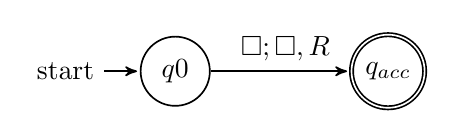
\begin{tikzpicture}[->,>=stealth',shorten >=1pt, auto, node distance=2cm, semithick]
    \tikzstyle{every state}=[text=black, fill=none]
    
    \node[initial,state] (q0)          {$q0$};
    \node[state,accepting]         (qacc) [right of=q0, xshift=20pt] {$q_{acc}$};
    
    \path (q0) edge  [bend left=0] node {\parbox{1cm}{$\square; \square, R$}} (qacc)
    ;
  \end{tikzpicture}
\end{center}

Example of string accepted: \\
Example of string rejected: \\


Implementation-level description

\vfill

High-level description

\vfill

\begin{center}
  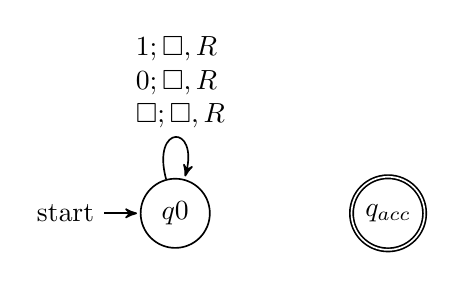
\begin{tikzpicture}[->,>=stealth',shorten >=1pt, auto, node distance=2cm, semithick]
    \tikzstyle{every state}=[text=black, fill=none]
    
    \node[initial,state] (q0)          {$q0$};
    \node[state,accepting]         (qacc) [right of=q0, xshift=20pt] {$q_{acc}$};
    
    \path (q0) edge  [loop above] node {\parbox{1cm}{$1; \square, R$\\$0; \square, R$\\$\square; \square, R$}} (q0)
    ;
  \end{tikzpicture}
\end{center}

Example of string accepted: \\
Example of string rejected: \\


Implementation-level description

\vfill

High-level description

\vfill

\newpage
 

\end{document}
